\documentclass{beamer}
\usepackage[utf8]{inputenc}
\usepackage[T1]{fontenc}
\usepackage{lipsum, lmodern}
\usepackage[scaled=.95]{helvet}% helvetica as the origin of arial
\usepackage[helvet]{sfmath}    % for the mathematical enviroments
\usepackage{braket}
\usepackage{physics}
\renewcommand{\familydefault}{\sfdefault}

%% ETH beamer theme
% Options: [default]
%   itemsblack/[itemsblue]: change color of bullets etc. to black/blue in itemize style environments
%   [titlesblack]/titlesblue: change color of frame titles/subtitles to black/blue
% \usetheme[itemsblack,titlesblack]{eth}
\usetheme{eth}

%% Theme uses ETH blue color by default. Can be changed to any color using this command: 
% \setbeamercolor{structure}{fg=blue}

%% Mandatory variables
\author{Matteo Bellino}
\title{Super-radiant and Sub-radiant Cavity Scattering by Atom Arrays}
\subtitle{Z. Yan \textit{et alii}, Phys. Rev. Lett \textbf{131} (2023)}
\date{February 27, 2025}

%% Optional variables
% \supervisor{Jane Smith} % for one supervisor
% \supervisors{Carol Foote, Jane Smith} % for multiple supervisors
%\projecttype{More Advanced Topics in Quantum Optics}

\begin{document}
\frame{\maketitle}
\begin{frame}{Definition}
	The term \alert{\textit{super-radiance}} was introduced by Dicke to refer to the phenomenon of coherent, constructive interference of the radiation emitted by a gas.
	The resulting intensity scales up quadratically in the number $N$ of sources.\newline\pause
	~\newline
	Here the same concept is adapted to the case of scattering by a linear chain of atoms, and complemented with the opposite case, \alert{\textit{sub-radiance}}, in which the scaling is sub-linear in $N$.
\end{frame}

\begin{frame}{Experimental setup}
	\begin{minipage}{\textwidth}
		\centering
		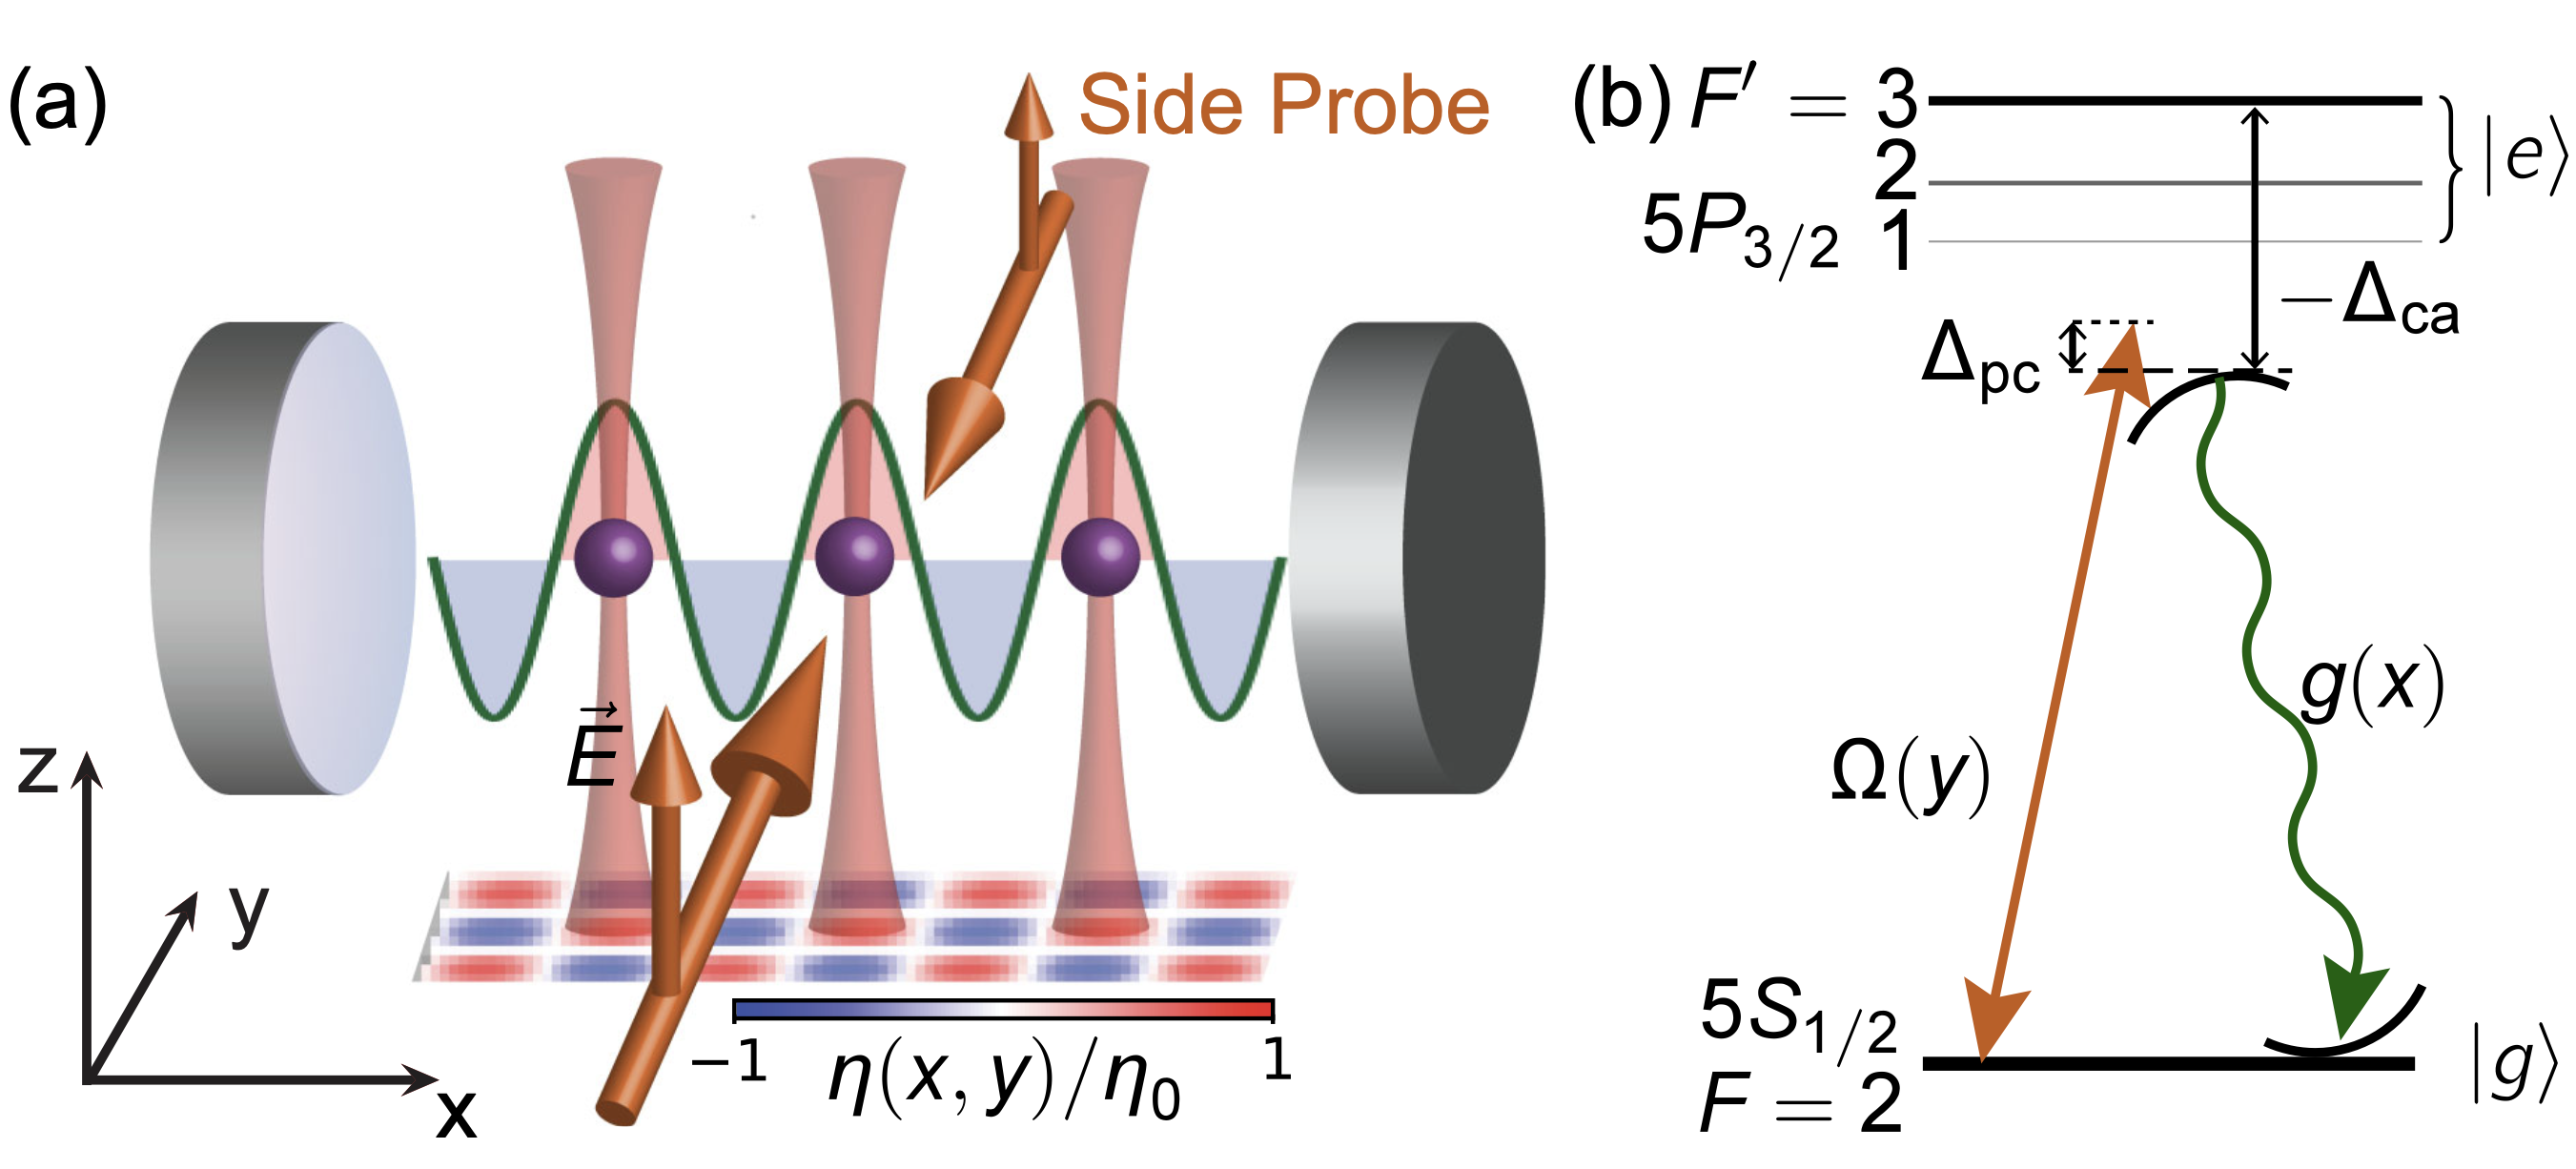
\includegraphics[width=0.8\textwidth]{Figure_1.png}
		\hspace{3em}
	\end{minipage}\newline
	\vspace{2em}
	\begin{minipage}{\textwidth}
		\begin{minipage}{0.57\textwidth}
			\begin{itemize}
				\item {\small 16 optical tweezers, $\sigma = 100\pm14\,$nm\pause}
				\item {\small cavity-atom coupling, $g(x)=g_0\cos(kx)$}\pause
				\item {\small laser-atom coupling, $\Omega(y)=\Omega_0\cos(ky)$}
			\end{itemize}
		\end{minipage}
		\begin{minipage}{0.42\textwidth}
			\centering
			$\,\lambda=780\,$nm\newline
			\alert{$\eta(x,y)=\eta_0\cos(kx)\cos(ky)$}
		\end{minipage}
	\end{minipage}
\end{frame}

\begin{frame}{Two-photons scattering}
	\begin{minipage}{0.4\textwidth}
		\centering
		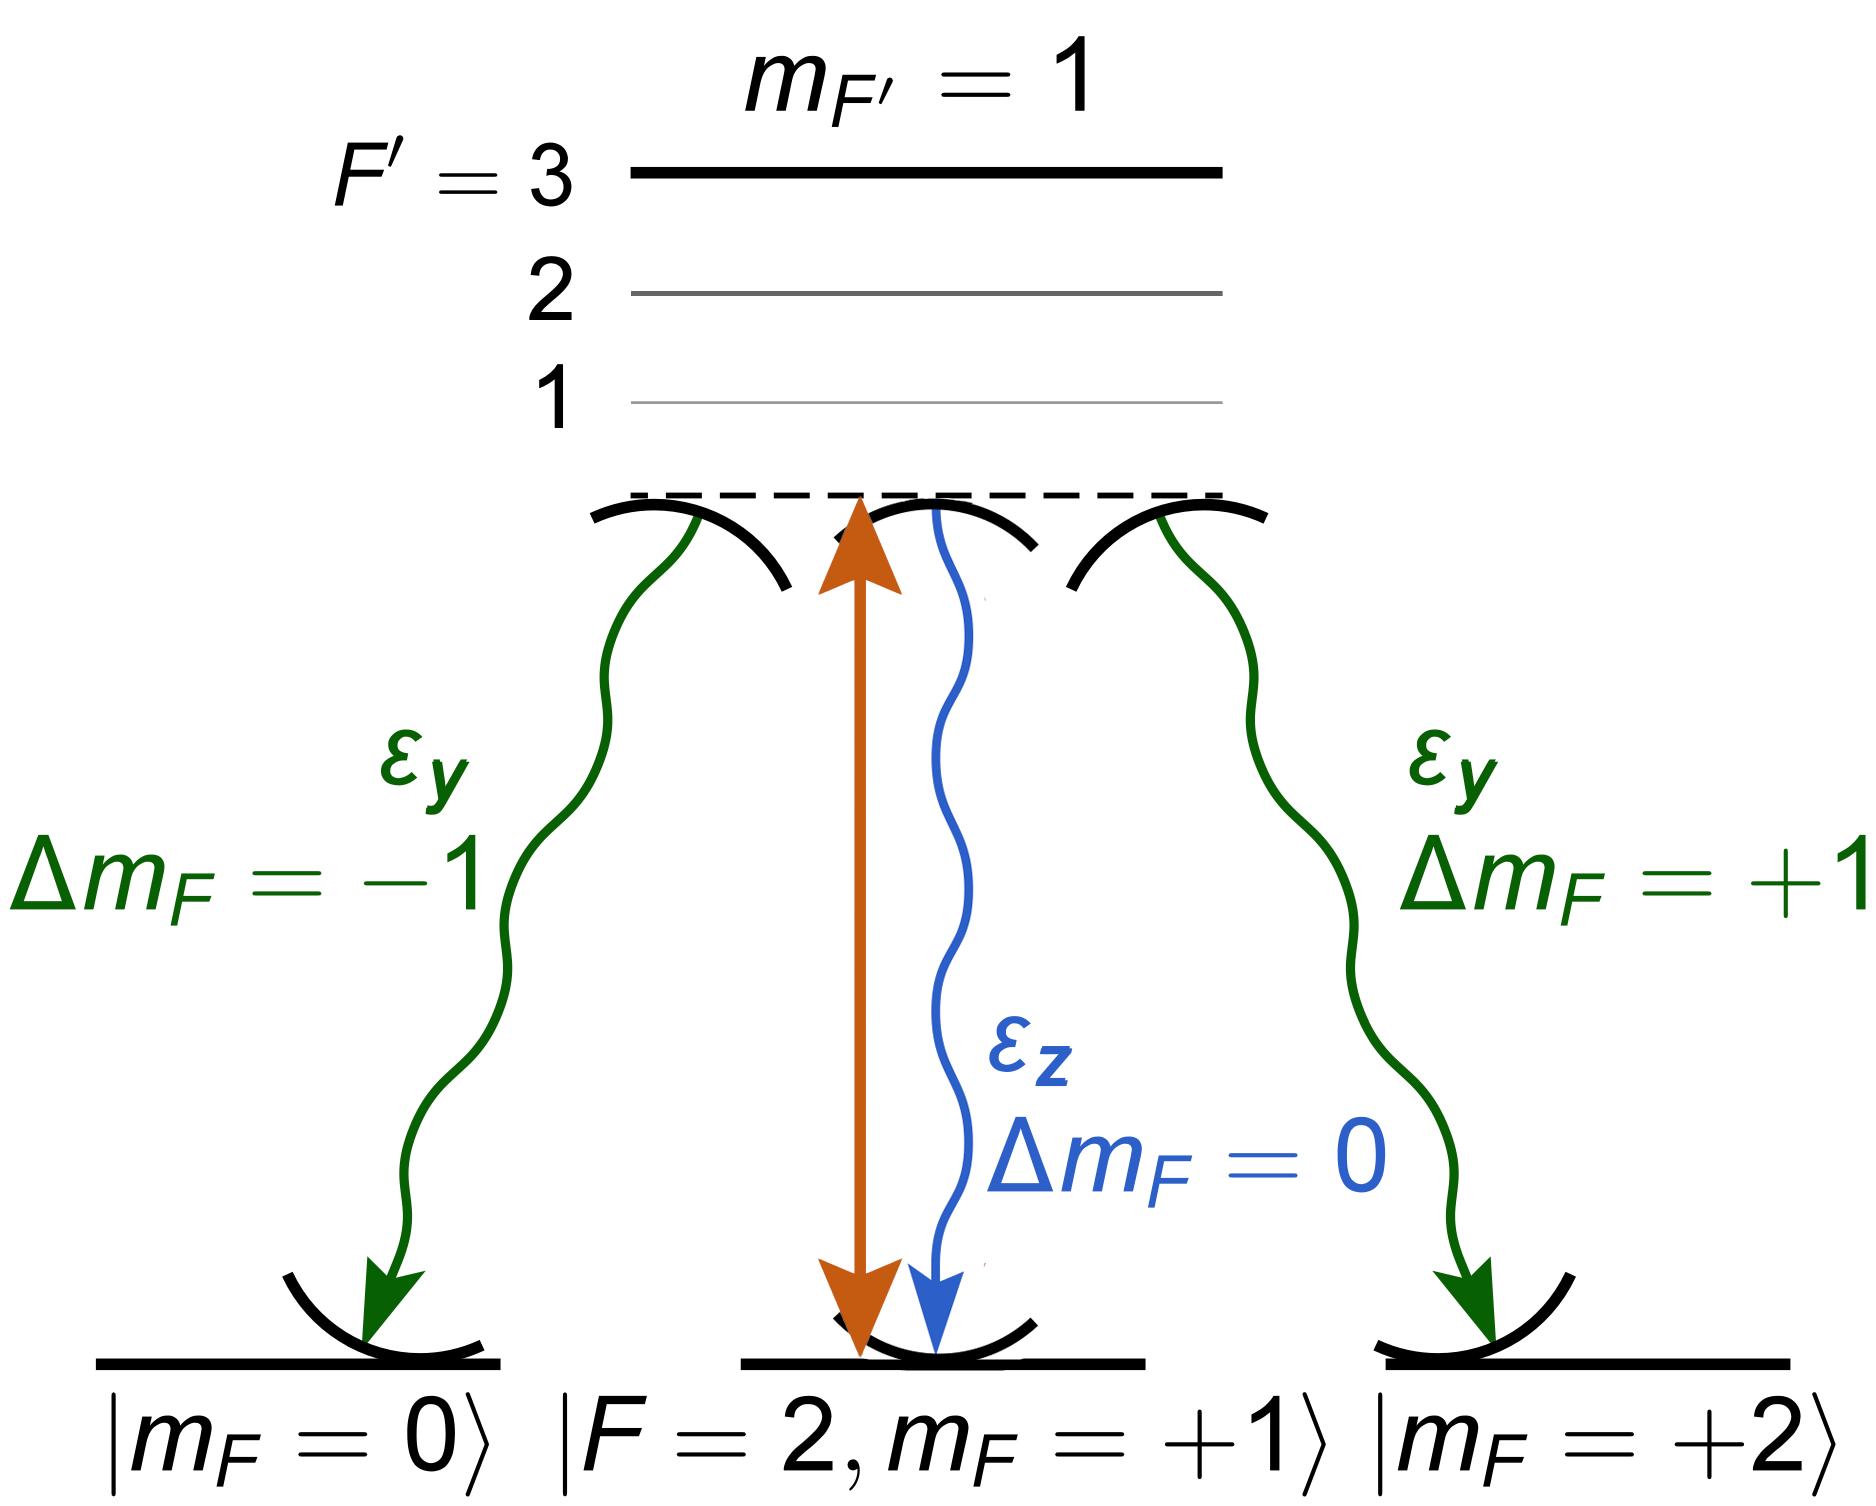
\includegraphics[width=\textwidth]{Figure_scattering_types.png}
	\end{minipage}
	\hfill
	\begin{minipage}{0.55\textwidth}
		\begin{center}
			Initial state: $\ket{m_{F,1},...,m_{F,i},...}\ket{0}_z\ket{0}_y$\pause
		\end{center}
		\vspace{2em}
		\textbf{Rayleigh scattering ($\Delta m_F=0$)}\\
		\vspace{-0.7em}
		\begin{equation*}
			\sum_{i=1}^N \eta^{Ray}_i\ket{m_{F,1},...,m_{F,i},...}\ket{1}_z\ket{0}_y\pause
		\end{equation*}\\~\\
		\textbf{Raman scattering ($\Delta m_F=\pm1$)}\\
		\vspace{-0.7em}
		\begin{equation*}
			\sum_{i=1}^N \eta^{Ram}_i\ket{m_{F,1},...,m_{F,i}\pm1,...}\ket{0}_z\ket{1}_y
		\end{equation*}
	\end{minipage}
\end{frame}

\begin{frame}{Two-photons scattering}
	The cavity photon number, distinguished on the scattering process (thus on polarization), is
	\begin{align*}
		n^{Ray}_N &\propto |\sum_{i=1}^N \eta^{Ray}_i|^2\\
		n^{Ram}_N &\propto \sum_{i=1}^N |\eta^{Ram}_i|^2
	\end{align*}
\end{frame}

\begin{frame}{Real-experiment complications}
	\begin{itemize}
		\item Atoms are not perfectly localised
		\vspace{-1em}
		\begin{equation*}
			n^{Ray}_N \propto \int...\dd{x_i}\dd{y_i}... \rho(x_i,y_i)...\; |\sum_{i=1}^N \eta^{Ray}_i|^2
		\end{equation*}
		\item The Rayleigh scattering amplitude of the i-th atom reads
		\vspace{-1em}
		\begin{equation*}
			\eta^{Ray}_i = \sum_{F'=1}^3\eta^{Ray}_0(m_{F,i},F')\cos(kx_i)\cos(ky_i)
		\end{equation*}
	\end{itemize}
\end{frame}

\begin{frame}{Magic detuning}
	\begin{align*}
		\text{At }\Delta_{ca}=-2\pi\times507\,\text{MHz}&\longrightarrow \eta^{Ray}_0(m_{F,i},F')=\eta^{Ray}_0(F')\\
		&\longrightarrow \eta^{Ram}_i=0 \quad\forall i
	\end{align*}
	Also, the atom-induced modifications of the cavity resonance can be neglected for large $|\Delta_{ca}|$.
\end{frame}

\end{document}

